\documentclass{article}
\usepackage[utf8]{inputenc}
\usepackage{geometry}
\geometry{
	a4paper,
	total={170mm,257mm},
	left=20mm,
	top=20mm,
}
\usepackage{graphicx}
\usepackage[dvipsnames]{xcolor}
\graphicspath{{images/}}
\usepackage{svg}
\usepackage{titling}
\usepackage[american,RPvoltages]{circuiTikz}
\usepackage{tikz, tikz-cd}
\usepackage{pgfplots}
\usepackage{siunitx}
\usepackage{float}
\usepackage{enumitem}
\usepackage{amsmath,amsfonts,stmaryrd,amssymb} % Math packages
\usepackage{tcolorbox}
\usepackage{pdfpages}
\usepackage{glossaries}
\usepgfplotslibrary{fillbetween}
\usetikzlibrary{intersections}
\title{El transistor como interruptor}
\author{Rodrigo Castillejos}
%\author{Belmont}
\date{Enero 2025}


\usepackage{fancyhdr}
\fancypagestyle{plain}{%  the preset of fancyhdr 
	\fancyhf{} % clear all header and footer fields
	\fancyfoot[L]{\thedate}
	\fancyhead[L]{Temporizador 555}
	\fancyhead[R]{\theauthor}
}
\makeatletter
\def\@maketitle{%
	\newpage
	\null
	\vskip 1em%
	\begin{center}%
		\let \footnote \thanks
		{\LARGE \@title \par}%
		\vskip 1em%
		%{\large \@date}%
	\end{center}%
	\par
	\vskip 1em}
\makeatother

\renewcommand{\figurename}{\textbf{Figura}}
%\usepackage[color=ForestGreen!15,angle=45]{draftwatermark}
%\SetWatermarkText{CONFIDENTIAL\\COPY FOR\\ POCA POCA}
%\SetWatermarkScale{2.5}

\usepackage{lipsum}  
%\usepackage{cmbright}
%\usepackage{mathpazo}
%\usepackage{ccfonts,eulervm}
 \usepackage[T1]{fontenc}
 \usepackage{ccfonts}
%\usepackage[math]{anttor}
%\usepackage{antpolt}
 %\usepackage{fouriernc}
%\usepackage[utopia]{mathdesign}
%---------------------------------------------------
\tikzset{flipflop myRS/.style={flipflop,
		 flipflop def={t1=R, t3=S, t6=Q, t4={\ctikztextnot{Q}}, tu={\ctikztextnot{RST}}, nu=1, n4=1 }}
	}
	
\tikzset{flipflop myFFRS/.style={flipflop,
		flipflop def={t1=R, t3=S, t6=Q, t4={\ctikztextnot{Q}}, n4=1 }}
}
%---------------------------------------------------
\setlength\parindent{0pt}

\newcommand{\drawpulse}[2][0]{% draw a pulse inside an empty source
	\begin{scope}[rotate=#1]
		\draw (#2.center) ++(-3mm, -2mm) -| ++(2mm,5mm)
		-- ++(2mm,0mm) |- ++(2mm, -5mm);
	\end{scope}
}
\begin{document}
	
\maketitle
	
\noindent\begin{tabular}{@{}ll}
Author & \theauthor\\
\end{tabular}
	
\section{El transistor de unión bipolar}
El transistor (una contracción para \textit{transfer resistor}) es un dispositivo semiconductor multiunión. Normalmente, el transistor es conectado con otros elementos de circuitos para lograr ganancia de voltaje, ganancia de corriente o ganancia de potencia. El transistor bipolar, llamado también transistor de unión bipolar (BJT), es uno de los dispositivos semiconductores más importantes, éste ha sido usado extensamente en circuitos de alta velocidad, circuitos analógicos y aplicaciones de potencia. Los dispositivos bipolares son dispositivos semiconductores en los cuales tanto los electrones como los huecos participan en el proceso de conducción. \\

El transistor bipolar fue inventado por un equipo de investigación en \textit{Bell Laboratoies} en 1947. Inicialmente el dispositivo tenía dos alambres de metal con puntos afilados haciendo contacto con un sustrato de germanio. Sin embargo, en transistores bipolares modernos, se reemplazó el germanio con silicio y los puntos de contactos fueron reemplazados con dos uniones $p-n$ acopladas en la forma de estructuras $p\textrm{-}n\textrm{-}p$ o $n\textrm{-}p\textrm{-}n$.

\subsection{Funcionamiento del transistor}
En la figura \ref{ch1f1} se muestra una perspectiva de la vista de un transitor $p\textrm{-}n\textrm{-}p$. El transistor se forma comenzando con un sustrato del tipo $p$, posteriormente se difunde térmicamente una región de tipo $n$ a través de una ventana de óxido en el sustrato tipo $p$. Posteriormente se difunde una región $p^+$ altamente dopada en la región tipo $n$.

\begin{figure}[H]
	\centering
	% trim=left botm right top
	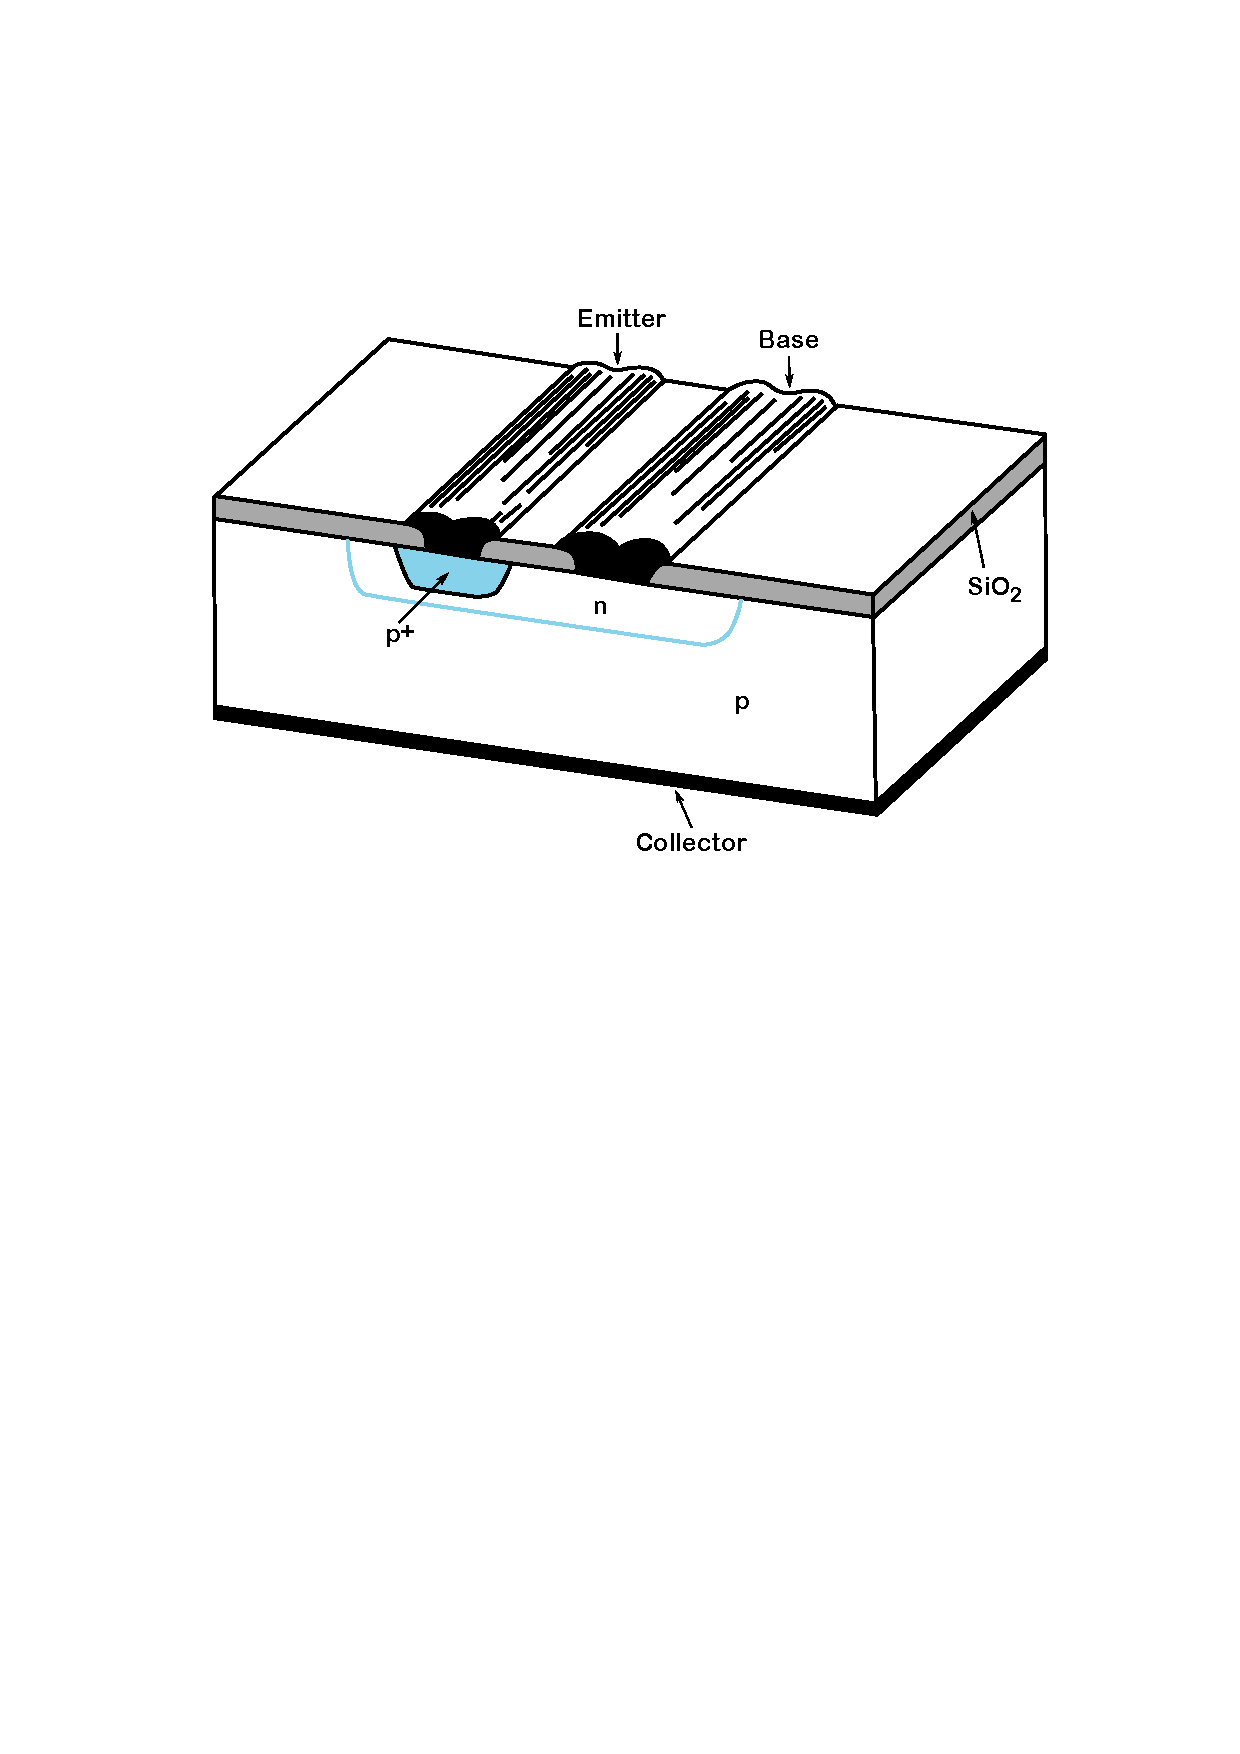
\includegraphics[clip, trim=2cm 15cm 3cm 5cm, width=0.7\textwidth]{Transistor perspective}
	\caption{Vista perspectiva de un transistor bipolar $pnp$}
	\label{ch1f1}
\end{figure}

\section{El transistor como interruptor}

\subsection{Transistor como interruptor ideal}
El transistor puede ser operado como un interruptor . Idealmente, si el transistor es polarizado en inversa puede operar como un interruptor abierto como se muestra en la figura \ref{ch2f1}(a). La condición de interruptor abierto, como se ilustra en la figura \ref{ch2f1}(a) se representa por el punto de operación $B$ en la recta de carga representada en la figura \ref{ch2f1}(c). Esta condición existe cuando la unión base emisor del transistor se polariza en inversa, y por lo tanto, la corriente de colector se reduce a cero.


\begin{figure}[H]
	\centering	
	\begin{tikzpicture}[scale=0.8]
		\ctikzset{bipoles/thickness=5}
		\ctikzset{monopoles/vcc/arrow={Stealth[width=6pt,length=9pt]}}
		\ctikzset{monopoles/vee/arrow={Stealth[width=6pt,length=9pt]}}
		\ctikzset{transistors/thickness=5}
		\draw (0,0) node[npn, anchor=B, xscale=1](Q){};
		\draw (Q.C) to[short, -*] ++(0,0.5) coordinate (p1)
		      to[R, l=$R_L$] ++(0,3) node[vcc](VCC){$+V_{CC}$};
		\draw (Q.B) to[short] ++(-2,0) to[V] node[left=15mm,above=7mm]{\textrm{polarización}} node[left=15mm,above=4mm]{\textrm{en inversa}} ++(0,-3) coordinate (g1) node[ground]{};
		\draw (Q.E) to[short] (Q.E |- g1) node[ground]{};
		\draw (p1) to[short, -o] ++(2,0) coordinate (p2);
		\draw (p2) to[open, -o, v=${V_o = V_{cc}}$] (p2 |- g1) node[ground]{};    
		
		\draw (0,0)++(4,0) node[]{$\Longrightarrow$};
		\draw (0,0)++(5,-1) to[cosw] node[right=3mm, below=5mm]{$B$} ++(0,3) node[above]{\textrm{OFF}};
		
		\draw (0,0)++(11,0) coordinate (a1) node[npn, anchor=B](Q2){};
		\draw (Q2.B) to[short] ++(-2,0)
		      to[V, invert] node[left=15mm,above=7mm]{\textrm{polarización}} node[left=15mm,above=4mm]{\textrm{en directa}} ++(0,-3) coordinate (r1) node[ground]{};
		\draw (Q2.E) to[short] (Q2.E |- r1) node[ground]{};
		\draw (Q2.C) to[short, -*] ++(0,0.5) coordinate (r2)
			  to[R, l=$R_L$] ++(0,3) node[vcc](VCC){$+V_{CC}$};
		\draw (r2) to[short ,-o] ++(2,0) coordinate (r3);
		\draw (r3) to[open, -o, v=${V_o = 0}$] (r3 |- r1) node[ground]{};
		
		\draw (a1)++(4,0) node[]{$\Longrightarrow$};
		\draw (a1)++(5,-1) to[ccsw] node[right=3mm, below=5mm]{$A$} ++(0,3) node[above]{\textrm{ON}};
		
		\draw (0,0)++(0,-4.5) node[below]{\textrm{(a) Transistor como interruptor abierto}};
		\draw (a1)++(0,-4.5) node[below]{\textrm{(b) Transistor como interruptor cerrado}};
		\draw (0,0)++(6,-13) node[below]{\textrm{(c) Curva característica ideal}};
		
		\pgfplotsset{width=9cm,height=7cm,compat=1.18}
		\begin{axis}[xshift=3cm,
			yshift=-12cm,
			clip=false,
			axis y line=left,
			axis x line=middle, 
			axis y line= center,
			xmin=0,xmax=5.5,
			ymin=0,ymax=1,
			xtick={0, 2.75,5},
			ytick={0.9,1},
			xticklabels={$0$,$V_{CE}$,$V_{CC}$},
			yticklabels={$\frac{V_{CC}}{R_L}$,$I_C$},
			]
			\addplot[line width=1pt,mark=none,const plot, color=magenta] coordinates {(0,0.9) (2,0.9)};
			\addplot[line width=1pt,mark=none,const plot, color=magenta] coordinates {(0,0.6) (3,0.6)};
			\addplot[line width=1pt,mark=none,const plot, color=magenta] coordinates {(0,0.3) (4,0.3)};
			\addplot[line width=1pt,mark=none,const plot, color=magenta] coordinates {(0,0) (5,0)};
			\addplot[line width=2pt,mark=none, color=cyan] coordinates {(0,0.9) (5,0)};
			\addplot[red, mark=*, only marks] coordinates {(0,0.9) (5,0)};
			\draw[Stealth-] (5, 0) -- (5.2, 0.1);
			\draw(5,0) node[right=3mm,above=5mm]{$B \,\, (OFF)$};
			\draw(2.75,0.6) node[right=4mm]{$I_B$};
			\draw[Stealth-] (0, 0.9) -- (0.2, 1);
			\draw(0,1) node[right=2mm]{$A \,\, (ON)$};
			\draw(5,0) node[right=8mm]{$I_B=0$};
		\end{axis}
	\end{tikzpicture}
	\caption{El transistor como interruptor ideal}	
	\label{ch2f1}
\end{figure}

El transistor conduce uando la unión base emisor del transistor se polariza en directa. Si la amplitud de dicha polarización es lo suficientemente grande, el transistor conducirá en saturación como se muestra en la figura \ref{ch2f1}(b). Cuando el transistor conduce estando en saturación la corriente de colector se encuentra limitada por el resistor $R_L$ ya que la resistencia vista por el transistor entre las terminales de colector y emisor es idealmente cero independientemente de la corriente de colector. \\

En una configuración del tipo de emisor común, la corriente de base $(I_B)$ controla la corriente de colector $(I_C)$. Debido a que $I_C = \beta I_B$, para un transistor ideal, una pequeña corriente de base puede controlar una gran corriente de colector. La corriente de base se determina por el voltaje a través de la unión base-emisor la cual controla la corriente de colector. La corriente de colector será de cero cuando el voltaje de entrada sea cero o cuando la unión base-emisor se polarice en inversa. Cuando el voltaje de entrada polarice en directa la unión base-emisor del colector ($\qty{0.7}{\volt}$ para un transistor de silicio), el transistor conducirá en saturación. De este manera, una pequeña incursión de voltaje ($0$ a $\qty{0.7}{\volt}$ para el transistor de silicio) es capaz de controlar una gran incursión de corriente de colector en la salida. \\

Refiérase a la figura de la figura \ref{ch2f1}(c). En el punto $A$ de la recta de carga, la corriente de colector es grande, pero el voltaje en la unión colector-emisor es cero. Por lo tanto, el transistor no disipa potencia cuando opera como un interruptor cerrado. En cambio, en el punto $B$ de la recta de carga, la corriente de colector es cero y el voltaje en la unión colector-emisor es $V_{cc}$. Por lo tanto, el transistor no disipa potencia cuando opera como un interuptor abierto. El transistor ideal, por lo tanto, puede manejar una gran cantidad de potencia hacia una carga sin disipar potencia.


 \subsection{Parámetros prácticos del transistor}
 La figura \ref{ch2f2} muestra la curva característica práctica de un transistor en emisor común. el área $I$ representa la región de operación de saturación. En esta región tanto la unión de emisor-base como la unión colector-base se encuentran polarizadas en directa. El área $II$ representa la región de operación activa del transistor. En esta área operan todos los amplificadores de clase A, donde la unión base-emisor es polarizada en directa y la unión colector-base es polarizada en inversa. El área $III$ representa la región de operación de corte. En esta área, la unión base-emisor y colector-base se encuentran polarizadas en inversa. 
 
\begin{figure}[H]
	\centering	
	\begin{tikzpicture}[scale=0.8]
		\pgfplotsset{width=9cm,height=7cm,compat=1.18}
		\begin{axis}[
			clip=false,
			axis y line=left,
			axis x line=middle, 
			axis y line= center,
			xmin=0,xmax=5.7,
			ymin=0,ymax=1.1,
			xtick={1,5},
			ytick={0.18,0.9,1.1},
			%xlabel=$V_{CE_{max}}$,
			xticklabels={$G$,$V_{cc}$},
			yticklabels={$D$,$\frac{V_{CC}}{R_L}$,$I_{C_{max}}$},
			]
			\addplot[name path=F, line width=1pt,mark=none, color=magenta, domain={0:1}]{0.72*x};
			\addplot[name path=G, line width=1pt,mark=none, color=magenta, domain={0:5}]{-0.18*x + 0.9};
			\addplot[name path=H, line width=1pt,mark=none, color=magenta, domain={0:4}]{0.045*x};
			\addplot[line width=1pt,mark=none, color=magenta, domain={4:4.5}]{0.045*x};
			\addplot[line width=1pt,mark=none, color=magenta, domain={0.135/0.72:4}]{0.045*x + 0.135};
			\addplot[line width=1pt,mark=none, color=magenta, domain={0.4:3.6}]{0.045*x + 0.27};
			\addplot[line width=1pt,mark=none, color=magenta, domain={0.6:3.2}]{0.045*x + 0.405};
			\addplot[line width=1pt,mark=none, color=magenta, domain={0.8:2.8}]{0.045*x + 0.54};
			\addplot[line width=1pt,mark=none, color=magenta, domain={1:2.4}]{0.045*x + 0.675};
			\addplot[line width=1pt,mark=none, dashed, color=magenta, domain={0.9:2.5}, restrict y to domain*=0:1.5]{0.2*(x-2.7)^2 + 0.45};
			\draw[name path=I] (0,0) -- (5,0);
			\addplot[fill=black, fill opacity=0.1] fill between [of=F and G, soft clip={domain=0:1}];
			\addplot[fill=black, fill opacity=0.1] fill between [of=H and I, soft clip={domain=0:5}];
			\addplot[color=black, dashed, thick] coordinates {(0, 0.18) (4,0.18)};
			\addplot[color=black, dashed, thick] coordinates {(4, 0.18) (4,0)};
			\addplot[color=black, dashed, thick] coordinates {(1, 0.72) (1,0)};
			\addplot[magenta, mark=*, only marks] coordinates {(0,0.9) (5,0) (1,0.72) (4,0.18) (2.5,0.45)};
			\draw (1,0.72) node[,left=2mm,above=2mm]{$A$};
			\draw (4.2,0.18) node[right=3mm]{$I_B=0$};
			\draw (2,0.7) node[right=9mm]{$I_B \, (mA)$};
			\draw (4,0.18) node[above]{$B$};
			\draw (5.7,0) node[right=1mm]{$V_{CE_{max}}$};
			\draw (0.1,0.6) node[right=1mm]{$I$};
			\draw (2.5,0.06) node[right=1mm]{$III$};
			\draw (1,0.4) node[right=3mm]{$II$};
		\end{axis}
	\end{tikzpicture}
	\caption{El transistor como interruptor ideal}	
	\label{ch2f2}
\end{figure}

\subsubsection{Operación del transistor en el modo activo (región II)}
De los tres modos de operación, el modo activo es el más importante. Esta situación se ilustra en la figura \ref{ch2f3} para el transistor $npn$. Se usan dos fuentes de voltaje externas (representadas como baterías) para establecer las condiciones de polarización requeridas para la operación en el modo activo. El voltaje $V_{BE}$ causa que la base de tipo $p$ esté a un potencial mayor que el emisor de tipo $n$, polarizando así en directa la unión base-emisor. El voltaje colector-base $V_{CB}$ causa que el colector de tipo $n$ se encuentre a un potencial mayor que la base de tipo $p$, polarizando así en inversa la unión colector-base.

\begin{figure}[H]
	\centering
	% trim=left botm right top
	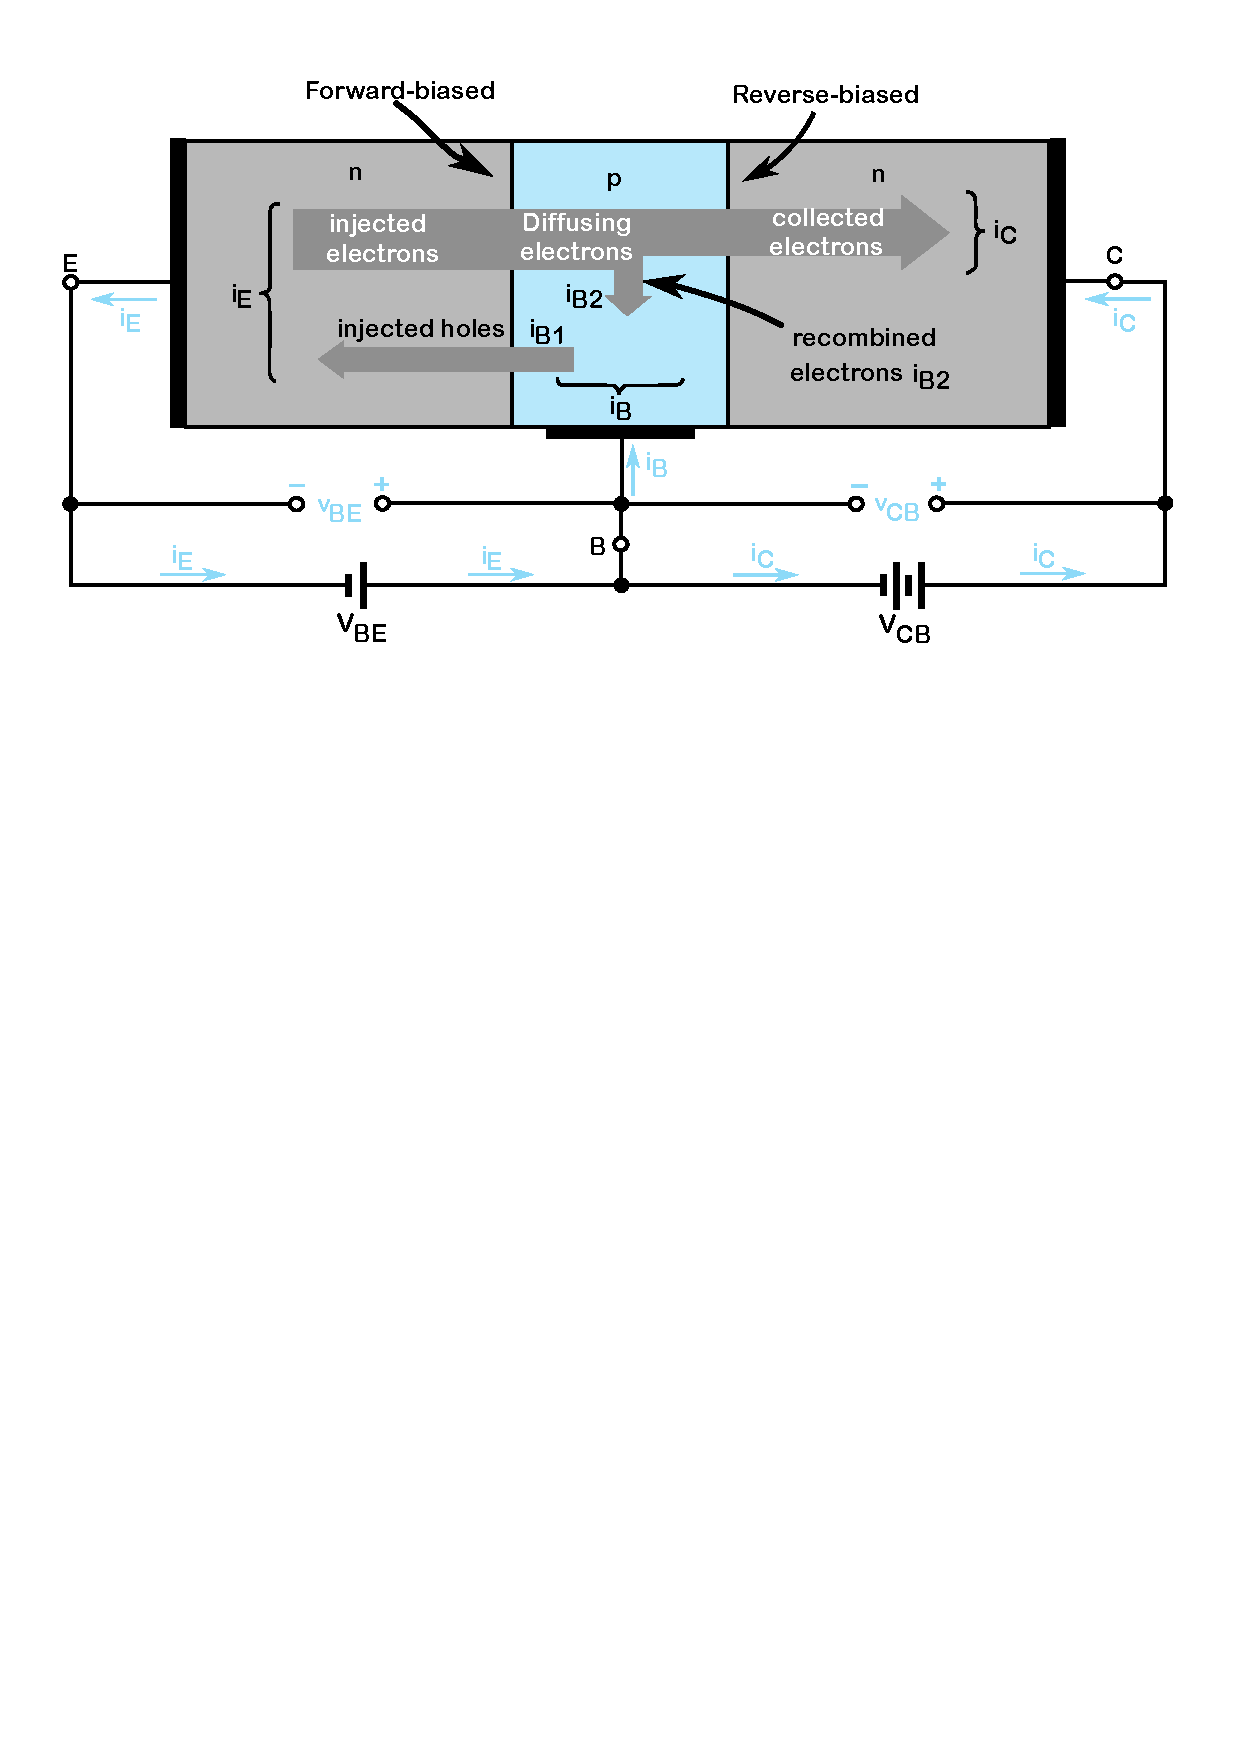
\includegraphics[clip, trim=1cm 18.5cm 0cm 1cm, width=0.9\textwidth]{transistor}
		\caption{El transistor como interruptor ideal}
		\label{fig3}
	\label{ch2f3}
\end{figure}

\begin{description}
	\item[Flujo de corrientes] La polarización en directa de la unión base-emisor causará un flujo de corriente a través de la unión. La corriente consistirá de dos componentes: electrones inyectados desde el emisor hacia la base y huecos inyectados desde la base hacia el emisor. Es altamente deseable que el primer componente (electrones fluyendo desde el amisor hacia la base) sea mucho mayor que el segundo componente (huecos fluyendo desde la base al emisor). Esto se logra fabricando el dispositivo con un emisor altamente dopado y una base ligeramente dopada, esto es, el dispositivo es diseñado para tener una alta densidad de electrones en el emisor y una baja densidad de huecos en la base.\\
	La corriente que fluye a través de la unión base-emisor constituirá la corriente de emisor $i_E$ donde la dirección de $i_E$ es hacia afuera de la terminal de emisor. Del estudio del flujo de corriente a través de una unión $pn$ polarizada en directa, sabemos que la magnitud del componente del electrón y el componente del hueco de $i_E$ será porporcional a $e^{v_{BE}/V_T}$, donde $v_{BE}$ es el voltaje en directo a través de la unión base-emisor y $V_T$ es el voltaje térmico (aproximadamente $\qty{25}{\milli \volt}$ a temperatura ambiente).
	
	\item[La corriente de colector] La corriente de colector es transportada por los electrones que alcanzan la región de colector . Su dirección será opuesta a la del flujo de electrones, entrnado por lo tanto  ala terminal de colector. Su magnitud será proporcional a $e^{v_{BE}/V_T}$, así
	\begin{align}
		i_C = I_S e^{v_{BE}/V_T}
	\end{align}
	Donde la constante de porporcionalidad $I_S$, como en el caso del diodo, es llamada la \textbf{corriente de saturación} y es un parámetro del transistor. Una importante observación a realizar es que $i_C$ es independiente del valor de $v_{CB}$.
	
	\item[La corriente de base] La figura 3 muestra que la corriente de base $i_B$ contiene dos componentes. La primera componente $i_{B1}$ es debido a los huecos inyectados desde la región de base hacia la corriente de emisor. Esta componente de corriente es proporcional a $e^{v_{BE}/V_T}$. La segunda componente de la corriente de base, $i_{B2}$, es debido a los huecos que tienen que ser alimentados por el circuito externo con el fin de reemplazar los huecos perdidos desde la base a través del proceso de recombinación. Debido a que $i_{B2}$ es proporcional al número de electrones inyectados en la base, también será proporcional a $e^{v_{BE}/V_T}$. Así, la corriente de base total $i_B = i_{B1} + i_{B2}$ será proporcional a $e^{v_{BE}/V_T}$ y puede ser expresada como una fracción de la corriente de colector $i_C$ como se muestra a continuación:
	\begin{align}
		i_B = \frac{i_C}{\beta}
	\end{align}
	Esto es
	\begin{align}
		i_B = \left( \frac{I_S}{\beta}\right)e^{v_{BE}/V_T}
	\end{align}
	Donde $\beta$ es un parámetro del transistor. Para transistores $npn$ modernos, $\beta$ se encuentra en el rango de 50 a 200, pero puede ser tan alto  como 1000 para dispositivos especiales. El valor de $\beta$ es altamente influenciado por dos factores:el \textit{ancho} de la región de base, $W$, y el dopaje relativo de la región de base y la región de emisor, $N_A/N_D$. Para obtener una $\beta$ alta (lo cual es altamente deseable dado que $\beta$ representa un parámetro de ganancia) la base debe ser delgada ($W$ pequeño) y ligeramente dopada y el emisor debe ser altamente dopado (haciendo $N_A/N_D$ pequeño)
	\item[La corriente de emisor] Dado que la corriente que entra en el transistor debe salir, y como se puede observar de la figura \ref{fig3}, la corriente de emisor $i_E$ es igual a la suma de la corriente de colector $i_C$ y la corriente de base $i_B$, esto es:
	\begin{align}
		i_E = i_C + i_B
	\end{align}
	El uso de las ecuaciones (2) y (4) produce
	\begin{align}
		i_E = i_C + \frac{i_C}{\beta} = \frac{\beta + 1}{\beta}i_C
	\end{align}
	Esto es
	\begin{align}
		i_E = \frac{\beta + 1}{\beta}I_Se^{v_{BE}/V_T}
	\end{align}	
\end{description}

\newpage

El punto $A$ de la recta de carga de la figura \ref{ch2f2} representa el punto de operación práctico del transistor como interuoptor cerrado mostrado en la figura \ref{ch2f1}(b). El voltaje colector-emisor no es cero en la recta de carga práctica, sino de $\qty{0.3}{\volt}$. Este voltaje se refiere como el voltaje colector-emisor en saturación el cual es simbolizado como $V_{CE_{sat}}$ y se expresa en volts.
El valor exacto para un transistor en específico es una función de la corriente de colector y puede variar en el rango de $\qty{0.1}{\volt}$ a $\qty{0.1}{\volt}$ \\

El punto $B$ de la recta de carga de la figura \ref{ch2f2} representa el punto de operación práctico para el transistor ilustrado en la figura \ref{ch2f1}(a). En este circuito, la unión base-emisor es inversamente polarizada, por lo tanto, la corriente de base es de cero. La corriente de colector, por otro lado, no es de cero, sino que tiene un valor finito (representado por el punto $D$ de la figura \ref{ch2f2}). Esta corriente de colector se produce por la corriente de saturación de colector en inversa (simbolizada como $I_{CBO}$). Debido a que el transistor está en una configuraciónd e emisor común, $I_{CBO}$ se amplifica por un factor de ($\beta + 1$). Por lo tanto, la corriente de colector en el punto $D$ es apreciable.

\subsection{El transistor ideal como interruptor saturado}
En un transistor como interruptor ideal saturado un pulso de voltaje controla el transistor. Para un claro entendimiento de este concepto, observe la figura \ref{ch2f1}(a) y (b), el cual ilustra un pulso de voltaje que ha sido simulado por dos baterías en los circuitos con estados $ON$ y $OFF$. La figura ilustra los pulsos de este voltaje rectangular que son aplicados como voltaje de control en el transistor. 

\begin{figure}[H]
	\centering	
	\begin{tikzpicture}[scale=0.8]
		\ctikzset{bipoles/thickness=5}
		\ctikzset{monopoles/vcc/arrow={Stealth[width=6pt,length=9pt]}}
		\ctikzset{monopoles/vee/arrow={Stealth[width=6pt,length=9pt]}}
		\ctikzset{transistors/thickness=5}
		\draw (0,0) node[npn, anchor=B, xscale=1](Q){};
		\draw (Q.C) to[short, -*] ++(0,0.5) coordinate (p1)
		to[R, l=$R_L$] ++(0,3) node[vcc](VCC){$+V_{CC}$};
		\draw (Q.B) to[R, l_=$R_1$] ++(-3,0) to[esource, name=pulse1, v<=$v_{in}$] ++(0,-3) coordinate (g1) node[ground]{};
		\draw (Q.E) to[short] (Q.E |- g1) node[ground]{};
		\draw (p1) to[short, -o] ++(2,0) coordinate (p2);
		\draw (p2) to[open, -o, v=$V_o$] (p2 |- g1) node[ground]{};    

		\drawpulse{pulse1};

		\pgfplotsset{width=9cm,height=4.5cm,compat=1.18}
		\begin{axis}[xshift=5cm,
			yshift=2.5cm,
			clip=false,
			axis y line=left,
			axis x line=middle, 
			axis y line= center,
			xmin=0,xmax=1,
			ymin=0,ymax=1,
			xtick={0},
			ytick={0},
			xticklabels={$$},
			yticklabels={$$},
			]
			\addplot[line width=2pt,mark=none,const plot, color=cyan] coordinates {(0,0.8) (0.2,0.8) (0.2,0) (0.4,0) (0.4,0.8) (0.6,0.8) (0.6,0) (0.8,0) (0.8,0.8) (0.9,0.8)};
			\draw (0,1) node[above]{$v_{in}$};
			\draw (1,0) node[right]{$t$};
		\end{axis}
		
		\begin{axis}[xshift=5cm,
			yshift=-1cm,
			clip=false,
			axis y line=left,
			axis x line=middle, 
			axis y line= center,
			xmin=0,xmax=1,
			ymin=0,ymax=1,
			xtick={0},
			ytick={0},
			xticklabels={$$},
			yticklabels={$$},
			]
			\addplot[line width=2pt,mark=none,const plot, color=cyan] coordinates {(0,0.5) (0.2,0.5) (0.2,0) (0.4,0) (0.4,0.5) (0.6,0.5) (0.6,0) (0.8,0) (0.8,0.5) (0.9,0.5)};
			\draw (0,1) node[above]{$i_B$};
			\draw (1,0) node[right]{$t$};
		\end{axis}
		
		\begin{axis}[xshift=5cm,
			yshift=-4.5cm,
			clip=false,
			axis y line=left,
			axis x line=middle, 
			axis y line= center,
			xmin=0,xmax=1,
			ymin=0,ymax=1,
			xtick={0.2,0.4},
			ytick={0},
			xticklabels={$t_1$,$t_2$},
			yticklabels={$$},
			]
			\addplot[line width=2pt,mark=none,const plot, color=cyan] coordinates {(0,0.9) (0.2,0.9) (0.2,0) (0.4,0) (0.4,0.9) (0.6,0.9) (0.6,0) (0.8,0) (0.8,0.9) (0.9,0.9)};
			\draw (0,1) node[above]{$i_B$};
			\draw (1,0) node[right]{$t$};
		\end{axis}
		
		\pgfplotsset{width=5cm,height=6cm,compat=1.18}
		\begin{axis}[xshift=-3cm,
			yshift=-10cm,
			clip=false,
			axis y line=left,
			axis x line=middle, 
			axis y line= center,
			xmin=0,xmax=0.5,
			ymin=0,ymax=1,
			xtick={0.1,0.2,0.3},
			ytick={0},
			xticklabels={$t_0$,$t_1$,$t_2$},
			yticklabels={$$},
			axis line style={draw=none},
			]
			\addplot[line width=2pt,mark=none,const plot, color=cyan] coordinates {(0,0) (0.1,0) (0.1,0.9) (0.2,0.9) (0.2,0) (0.3,0) (0.3,0.9) (0.35,0.9)};
			\draw (0,0) node[left]{$OFF$};
			\draw (0,0.9) node[left]{$ON$};
			\draw (0,0.45) node[left]{$\Delta I_C$};
		\end{axis}
		
		\pgfplotsset{width=7cm,height=6cm,compat=1.18}
		\begin{axis}[xshift=3cm,
			yshift=-10cm,
			clip=false,
			axis y line=left,
			axis x line=middle, 
			axis y line= center,
			xmin=0,xmax=5.5,
			ymin=0,ymax=1,
			xtick={0.4,5},
			ytick={0.1,0.9},
			xticklabels={$V_{CE_{(sat)}}$,$V_{cc}$},
			yticklabels={$I_{C} = I_{CO}(h_{FE} + 1)$,$\frac{V_{cc}}{R_L}$},
			%axis line style={draw=none},
			]
			\addplot[line width=1pt,mark=none, color=magenta, domain={0:0.4}]{2.07*x};
			\addplot[line width=1pt,mark=none, color=magenta] coordinates {(0.4,0.828) (2.5,0.85)};
			\addplot[name path=G, line width=1pt,mark=none, color=magenta, domain={0:5}]{-0.18*x + 0.9};
			\addplot[name path=G, line width=1pt,mark=none, color=magenta, domain={0:5.5}]{0.01818*x};
			\draw (0,1) node[above]{$I_C \,, (mA)$};
			\draw (5.5,0) node[right]{$V_{CE} \, (V)$};
			\draw (2.5,0.85) node[right]{$I_B = \frac{I_C}{h_{FE_{(min)}}}$};
			\draw (5.5,0.1) node[above]{$I_B = 0$};
		\end{axis}
		
		\pgfplotsset{width=5cm,height=6cm,compat=1.18}
		\begin{axis}[xshift=12cm,
			yshift=-10cm,
			clip=false,
			axis y line=left,
			axis x line=middle, 
			axis y line= center,
			xmin=0,xmax=0.5,
			ymin=0,ymax=1,
			xtick={0.1,0.2,0.3},
			ytick={0},
			xticklabels={$t_0$,$t_1$,$t_2$},
			yticklabels={$$},
			axis line style={draw=none},
			]
			\addplot[line width=2pt,mark=none,const plot, color=cyan] coordinates {(0,0) (0.1,0) (0.1,0.9) (0.2,0.9) (0.2,0) (0.3,0) (0.3,0.9) (0.35,0.9)};
			\draw (0,0) node[left]{$OFF$};
			\draw (0,0.9) node[left]{$ON$};
			\draw (0,0.45) node[left]{$\Delta I_B$};
		\end{axis}
	\end{tikzpicture}
	\caption{El transistor como interruptor ideal}	
	\label{ch2f4}
\end{figure}

\subsection*{ejemplo 2.1}
Determine los parámetros necesarios para el transistor como interruptor que se muestra en la figura \ref{ch2f4}. El circuito tiene las siguientes características:
\begin{align}
	V_o = \qty{20}{\volt}_p \nonumber \\
	v_{in} = \qty{5}{\volt}_p \nonumber \\
	I_C = \qty{20}{\milli \ampere} \nonumber
\end{align}

Asumiendo un transistor ideal de silicio NPN con las siguientes especificaciones:

\end{document}